An important factor when deciding whether to purchase any type of vehicle is access to the corresponding fuel source. However, this consideration tends to be less critical for conventional vehicles, as their significantly greater range compared to EVs reduces dependency on frequent refueling infrastructure. Figure \ref{fig: charg_stat} demonstrates the number of charging stations per 100,000 inhabitants.

As of October 1st, 2023, there are approximately 108,000 public charging points across Germany, including around 21,000 fast charging stations. The previous government coalition had set an ambitious goal of expanding the charging infrastructure to one million stations by 2030. Once again, the most densely covered regions are found in the South—particularly in Bavaria and Baden-Württemberg, while the eastern states continue to lag behind in comparison to the West \cite{DeAtlasCharge}.
\begin{figure}[H]
	\begin{center}
		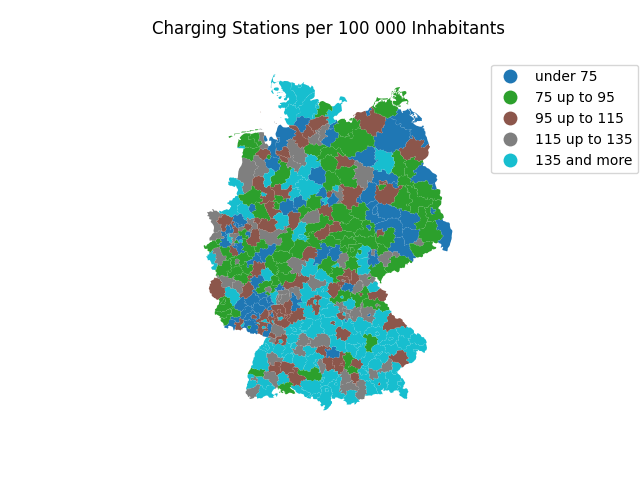
\includegraphics[width=\linewidth]{images/Charging_stations}
		\caption{Distribution of Charging Station Across German District}
		\label{fig: charg_stat}
		\captionsetup{font={footnotesize,bf,it}}
		\caption*{Data: Deutschlandatlas, \cite{DeAtlasEVXLSX} \\
  				Map: BKG, \cite{BKG} } 
	\end{center} 
\end{figure}
The calculated means of charging stations across different administrative categories (see Fig. \ref{fig: mean_charg}) show that urban districts have greater access to charging infrastructure. The 
\begin{figure}[H]
	\begin{center}
		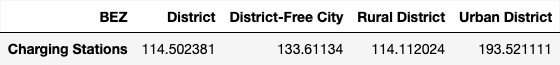
\includegraphics[width=\linewidth]{images/Charg_mean.png}
	\end{center}
	\caption{Distribution of Charging Stations}
	\label{fig: mean_charg}
\end{figure}
The calculated means of charging stations across different administrative groups show that urban districts have significantly greater access to charging infrastructure, s. Fig. \ref{fig: mean_charg}. This disparity likely reflects differences in population density, investment priorities, and the broader push for urban sustainability